	 \subsection{Integración con grub y división en módulos}

	Utilizamos grub en el nivel mas bajo del booteo para lograr un contexto inicial estable y que posibilitara la ejecución del trabajo practico desde un pendrive usb.\\

	Grub permite iniciar un kernel por medio de una especificación publicada en la web, en la que se detalla un contrato que debe cumplir tanto el kernel a iniciar como grub, entre ellas, un header que debe contener el ejecutable del kernel para ser identificado por grub como un sistema operativo, y por otro lado, las obligaciones que debe cumplir grub al entregarle el control a dicho kernel, es decir, un contexto determinado: selectores de código y datos válidos, registros de propósito general con valores específicos, etc.\\
	(\url{http://www.gnu.org/software/grub/manual/multiboot/multiboot.html})\\

	Esta revisión de grub no permite cargar ejecutables compilados en 64 bits de manera sencilla, por este motivo decidimos que lo mejor era utilizar a una herramienta provista por grub, llamada carga de módulos, que nos permitió cargar distintas partes no críticas del sistema por encima del primer mega de memoria y tener en un mapa de memoria provisto por grub, las posiciones exactas en la RAM de dichos módulos.\\ 

	Junto con la carga de módulos y el booteo del BSP, se prepara el entorno para el booteo en etapas de los AP.\\
	\begin{itemize}
		\item \textbf{Niveles de booteo del BSP y preparación del entorno de inicio de los AP:} 
			\begin{enumerate}
				\item Grub inicializa la máquina a un estado conocido y otorga el control al loader de nivel 1 del BSP pasándole por parámetros estructuras de grub con información del sistema.
				\begin{enumerate}
					\item Se realizan validaciones requeridas por la especificación multiboot, verificación de firmas, etc.
					
					\item Se obtienen de la metadata provista por grub las posiciones de memoria donde están cargados los módulos, ellos son:
					\vspace{0.1cm}
					\begin{description}
						\item [kernel64.bin64:] \hfill \\
							Módulo compilado en formato binario plano de 64 bits que contiene el segundo nivel de booteo del BSP.
						\item [ap\_full\_code.bin64:] \hfill \\
							Módulo compilado en formato binario plano de 64 bits que contiene el código del segundo nivel de booteo de los Application Processors.
						\item [ap\_startup\_code:] \hfill \\
							Módulo compilado en formato binario de 32 bits que contiene el código de inicio del AP en modo real y el primer stage de booteo a modo protegido.
					\end{description}
					\vspace{0.5cm}
					
					\item Los Application Processors inician en modo real, es por esto que deben comenzar su ejecución por debajo del primer mega de memoria principal. Por este motivo se copia el módulo ap\_startup\_code a una dirección arbitraria alineada a página 0x2000.
					\vspace{0.1cm}
					\item Como los AP comienzan su ejecución por debajo del primer mega, esto hace posible la superposición de código con grub y otras estructuras del kernel, para evitarlo, minimizamos el tamaño del startup de modo real del ap, haciendo lo antes posible un salto a un loader de nivel 2 por encima del mega, este loader de nivel 2 es ap\_full\_code.bin64.
					\vspace{0.1cm}
					\item Al tener el Application Processor que hacer un salto entre los dos niveles de booteo, se le inyecta al primer módulo la dirección donde esta cargado el segundo nivel de booteo.
					\vspace{0.1cm}
					\item Finalmente, se realiza un salto en la ejecución a donde comienza el modulo kernel64.bin64 donde el BSP finaliza la inicializacion del contexto hasta modo largo de 64 bits y enciende a los demás núcleos del sistema.
				\end{enumerate}
			\end{enumerate}
	\end{itemize}

	\subsubsection{Booteo e integración con grub: Mapa de memoria: Memoria baja y módulos en memoria alta}

	\begin{center}
		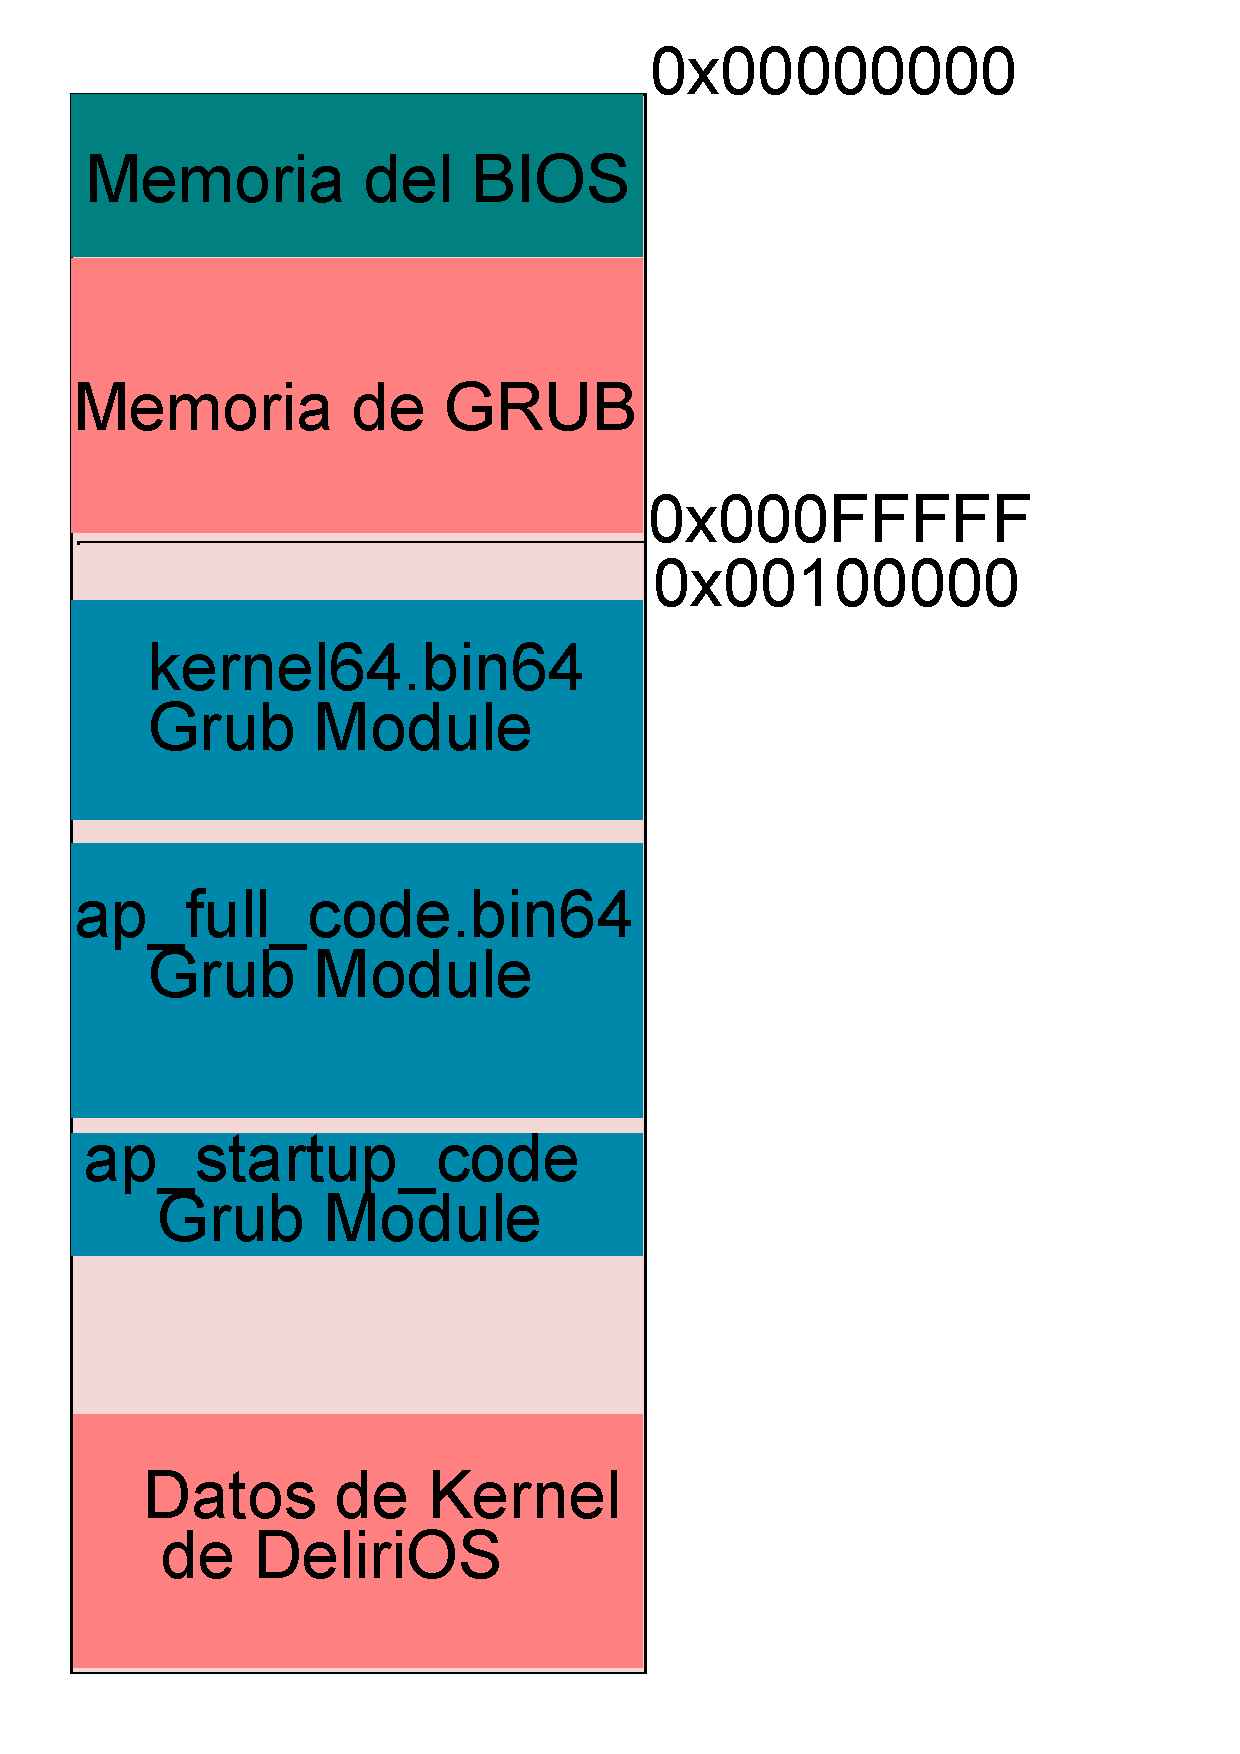
\includegraphics[height=7cm]{images/modules-map.pdf} 
	\end{center}
	\subsubsection{Booteo e integración con grub: Diagrama de interacción entre los niveles de Booteo e inyección de datos}

	\begin{center}
		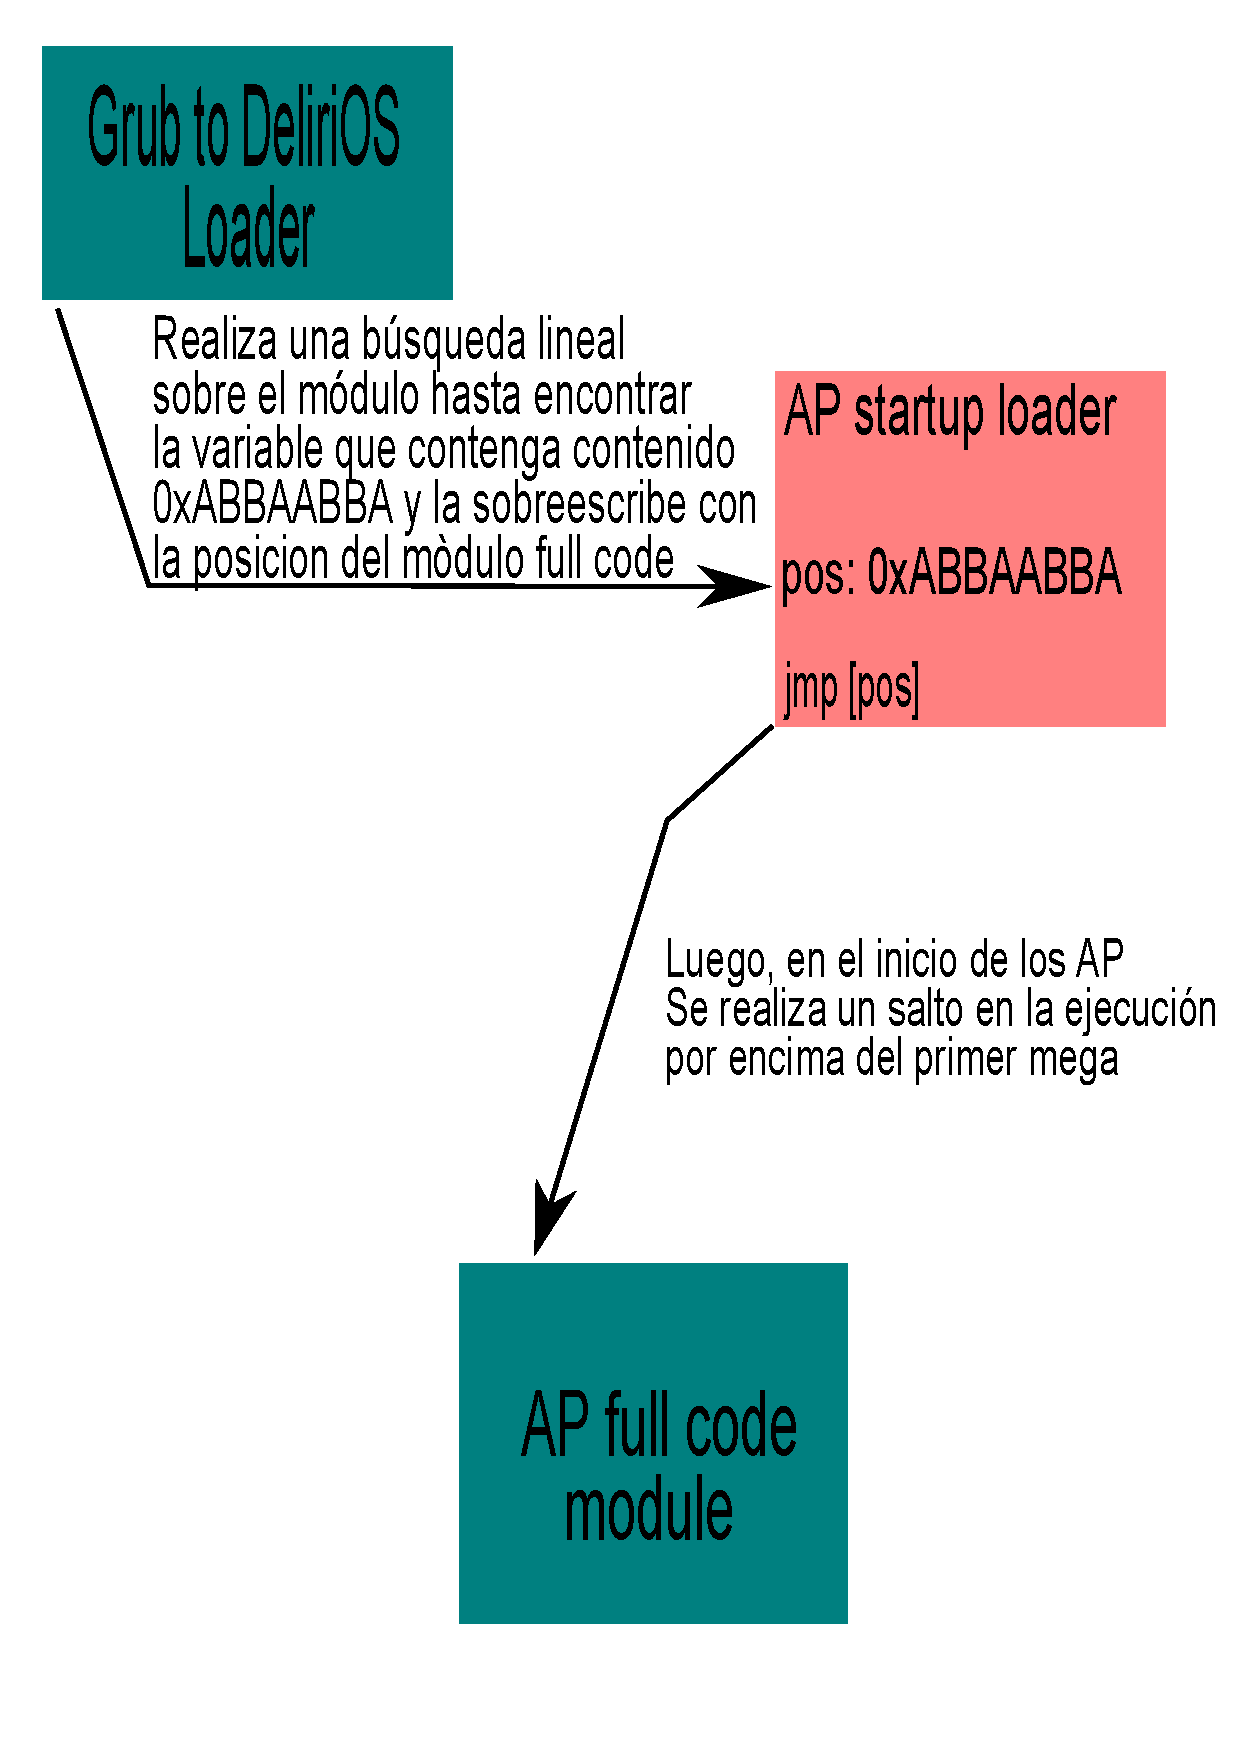
\includegraphics[height=12cm]{images/modules-diagram.pdf} 
	\end{center}

	\newpage

	\subsubsection{Niveles de booteo del BSP}

	\begin{center}
		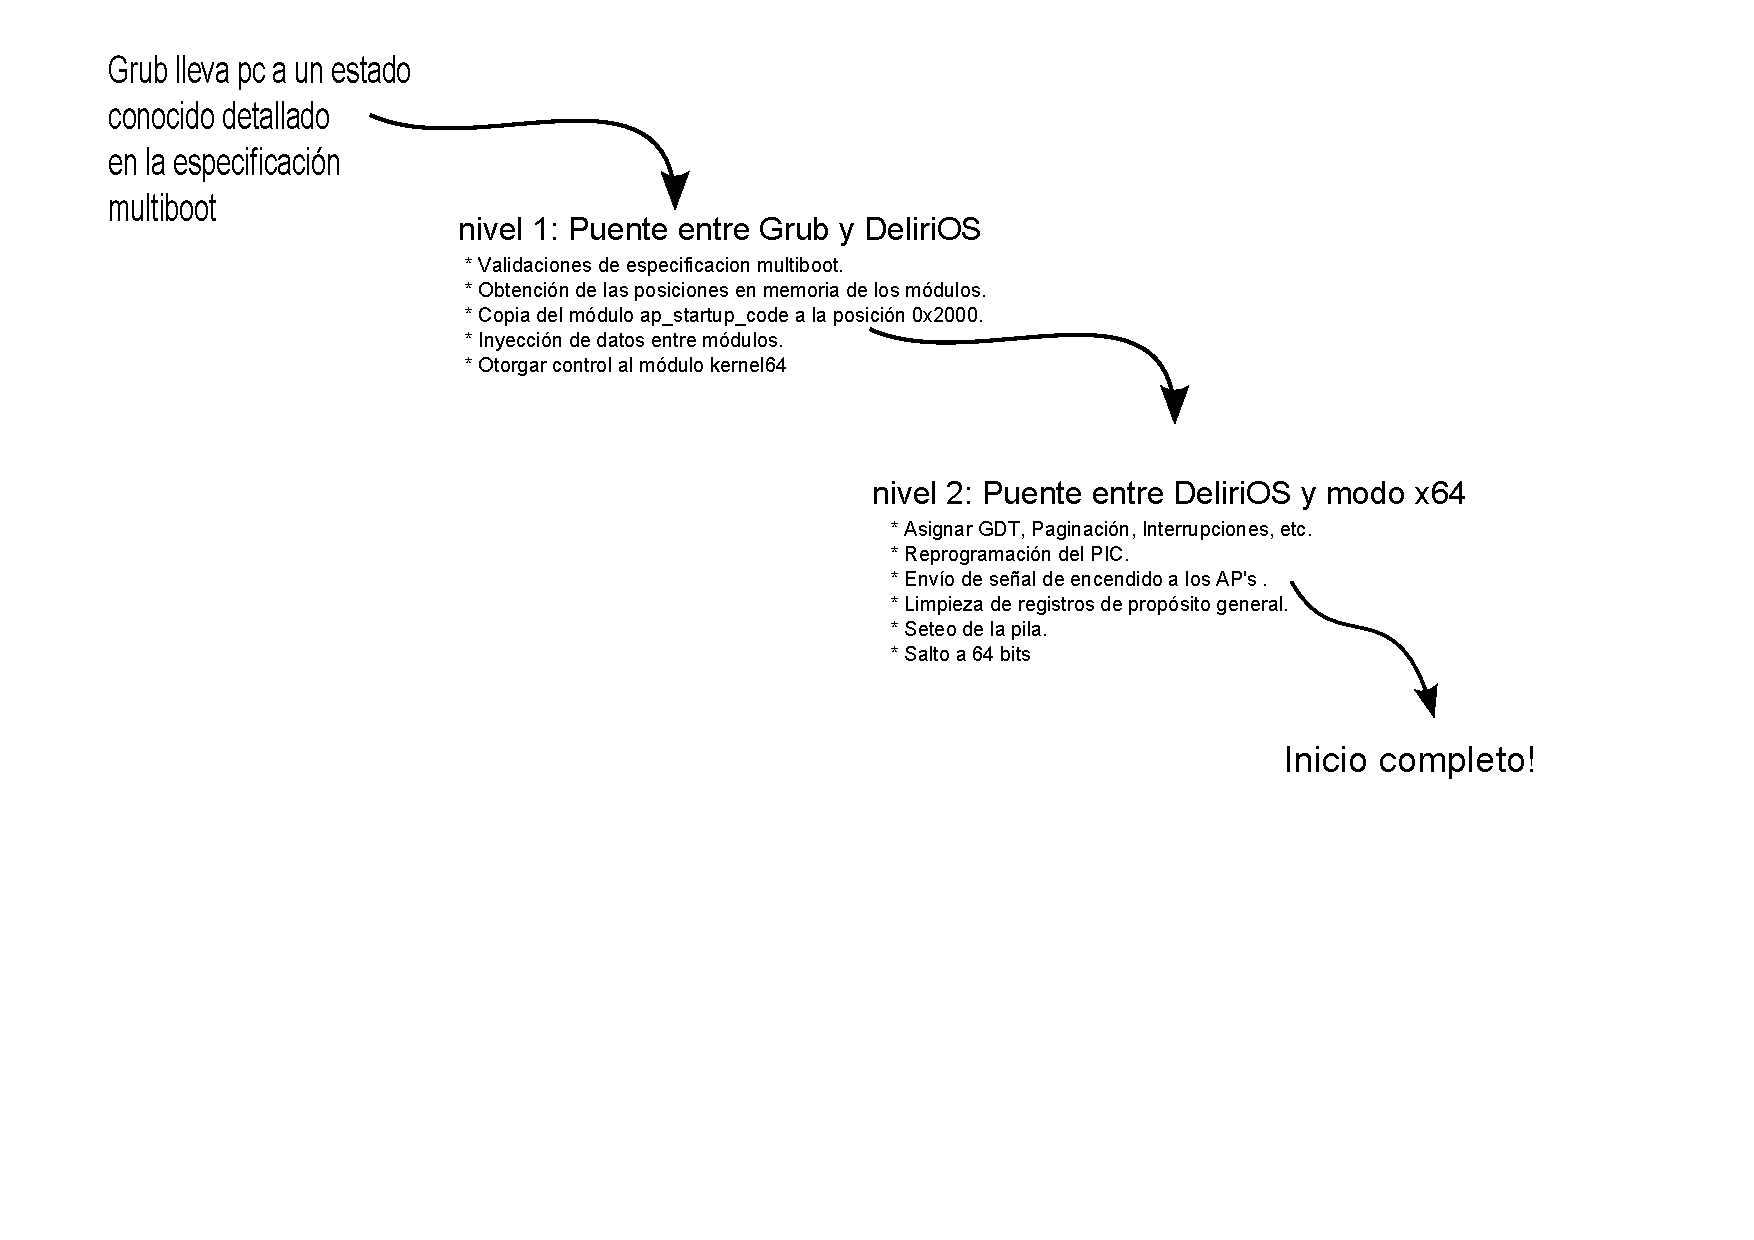
\includegraphics[height=14cm]{images/bsp-stages-diagram.pdf} 
	\end{center}
	
	\subsubsection{Niveles de booteo del AP}

	\begin{center}
		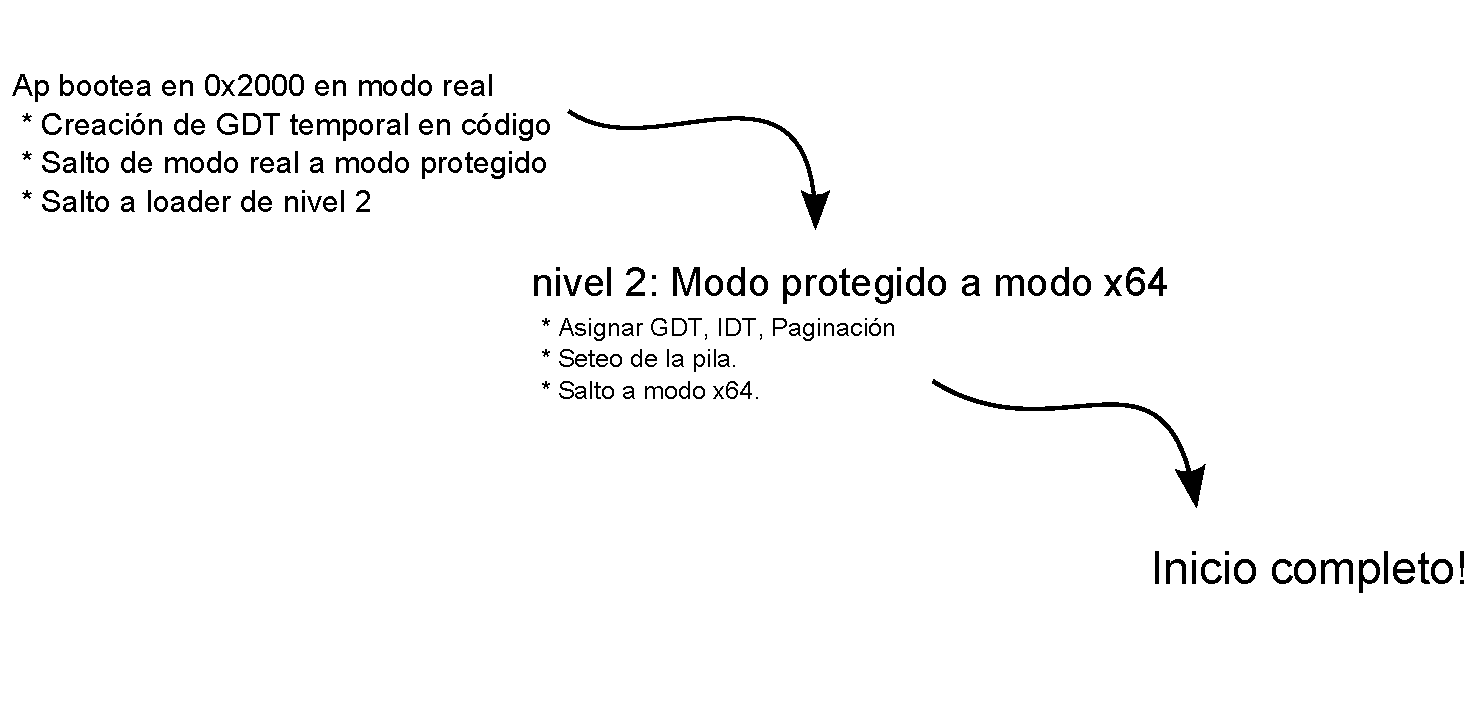
\includegraphics[height=8cm]{images/ap-stages-diagram.pdf} 
	\end{center}

